%
% hexagon1.tex -- Koordinaten 
%
% (c) 2019 Prof Dr Andreas Müller, Hochschule Rapperswil
%
\documentclass[tikz]{standalone}
\usepackage{amsmath}
\usepackage{times}
\usepackage{txfonts}
\usepackage{pgfplots}
\usepackage{csvsimple}
\usetikzlibrary{arrows,intersections,math}
\begin{document}
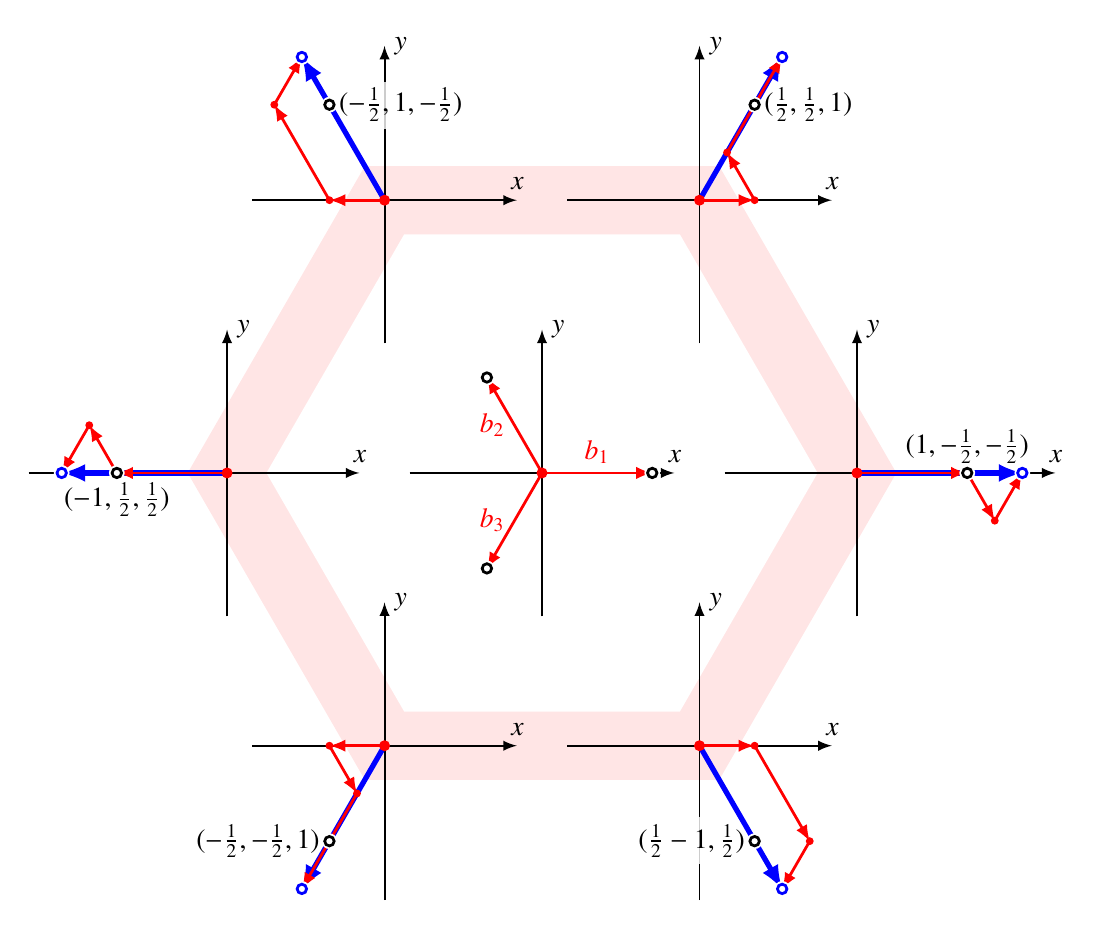
\begin{tikzpicture}[>=latex]

\def\a{1.4}

\def\punkt#1#2{
        \fill[color=white] ({#1},{#2}) circle[radius=0.1];
        \draw[line width=1pt] ({#1},{#2}) circle[radius=0.06];
}

\def\punktblau#1#2{
        \fill[color=white] ({3*#1/2},{3*#2/2}) circle[radius=0.1];
        \draw[line width=1pt,color=blue] ({3*#1/2},{3*#2/2}) circle[radius=0.06];
}

\def\outerradius{4.5}
\fill[color=red!10] 
	(\outerradius,0)--
	({\outerradius*cos(60)},{\outerradius*sin(60)})--
	({\outerradius*cos(120)},{\outerradius*sin(120)})--
	(-\outerradius,0)--
	({\outerradius*cos(240)},{\outerradius*sin(240)})--
	({\outerradius*cos(300)},{\outerradius*sin(300)})--cycle;

\def\innerradius{3.5}
\fill[color=white] 
	(\innerradius,0)--
	({\innerradius*cos(60)},{\innerradius*sin(60)})--
	({\innerradius*cos(120)},{\innerradius*sin(120)})--
	(-\innerradius,0)--
	({\innerradius*cos(240)},{\innerradius*sin(240)})--
	({\innerradius*cos(300)},{\innerradius*sin(300)})--cycle;

%\foreach \p in {30,90,...,330}{
%	\draw[color=gray!20,line width=2pt] (0,0)--
%		({(\outerradius+\a)*cos(\p)},{(\outerradius+\a)*sin(\p)});
%}

\draw[->,line width=0.7pt] ({-1.2*\a},0)--({1.2*\a},0)
	coordinate[label={$x$}];
\draw[->,line width=0.7pt] (0,{-1.3*\a})--(0,{1.3*\a})
	coordinate[label={right:$y$}];
\foreach \p in {0,120,240}{
	\draw[->,line width=1pt,color=red] (0,0)--({\a*cos(\p)},{\a*sin(\p)});
	\punkt{\a*cos(\p)}{\a*sin(\p)}
}
\node[color=red] at ({\a/2},0) [above] {$b_1$};
\node[color=red] at ({-\a/4},{\a*sqrt(3)/4}) [left] {$b_2$};
\node[color=red] at ({-\a/4},{-\a*sqrt(3)/4}) [left] {$b_3$};
\fill[color=red] (0,0) circle[radius=0.07];

\begin{scope}[xshift=4cm]
	\draw[->,line width=0.7pt] ({-1.2*\a},0)--({1.8*\a},0)
		coordinate[label={$x$}];
	\draw[->,line width=0.7pt] (0,{-1.3*\a})--(0,{1.3*\a})
		coordinate[label={right:$y$}];
	\draw[->,line width=1.9pt,color=blue] (0,0)
		--({3*\a/2},0);
	\draw[->,line width=1pt,color=red] (0,0)--({\a},0);
	\draw[->,line width=1pt,color=red] ({\a},0)
		--({5*\a/4},{-\a*sqrt(3)/4});
	\fill[color=red] ({5*\a/4},{-\a*sqrt(3)/4}) circle[radius=0.05];
	\draw[->,line width=1pt,color=red] ({5*\a/4},{-\a*sqrt(3)/4})
		--({3*\a/2},0);
	\node at ({\a},0) [above] {$(1,-\frac12,-\frac12)$};
	\punkt{\a*cos(0)}{\a*sin(0)}
	\punktblau{\a*cos(0)}{\a*sin(0)}
	\fill[color=red] (0,0) circle[radius=0.07];
	%\node[color=red] at ({\a/2},0) [above] {$b_1$};
\end{scope}

\begin{scope}[xshift=2cm,yshift=3.464cm]
	\draw[->,line width=0.7pt] ({-1.2*\a},0)--({1.2*\a},0)
		coordinate[label={$x$}];
	\draw[->,line width=0.7pt] (0,{-1.3*\a})--(0,{1.4*\a})
		coordinate[label={right:$y$}];
	\draw[->,line width=1.9pt,color=blue] (0,0)
		--({3*\a/4},{3*\a*sqrt(3)/4});
	\draw[->,line width=1pt,color=red] (0,0)--({0.5*\a},0);
	\fill[color=red] ({0.5*\a},0) circle[radius=0.05];
	\draw[->,line width=1pt,color=red] ({\a/2},0)
		--({\a/4},{0.5*\a*sqrt(3)/2});
	\fill[color=red] ({\a/4},{0.5*\a*sqrt(3)/2}) circle[radius=0.05];
	\draw[->,line width=1pt,color=red] ({\a/4},{\a*sqrt(3)/4})
		--({3*\a/4},{3*\a*sqrt(3)/4});
	\node at ({\a/2},{\a*sqrt(3)/2}) [right]
		{$\textstyle(\frac12,\frac12,1)$};
	\punkt{\a*cos(60)}{\a*sin(60)}
	\punktblau{\a*cos(60)}{\a*sin(60)}
	\fill[color=red] (0,0) circle[radius=0.07];
	%\node[color=red] at ({\a/2},0) [above] {$b_1$};
	%\node[color=red] at ({\a-\a/4},{\a*sqrt(3)/4}) [right] {$b_2$};
\end{scope}

\begin{scope}[xshift=-2cm,yshift=3.464cm]
	\draw[->,line width=0.7pt] ({-1.2*\a},0)--({1.2*\a},0)
		coordinate[label={$x$}];
	\draw[->,line width=0.7pt] (0,{-1.3*\a})--(0,{1.4*\a})
		coordinate[label={right:$y$}];
	\fill[color=white] (-0.1,0.9) rectangle (0.1,1.5);
	\draw[color=gray!40,line width=0.7pt] (0,0.9)--(0,1.5);
	\draw[->,line width=1.9pt,color=blue] (0,0)
		--({-3*\a/4},{3*\a*sqrt(3)/4});
	\draw[->,line width=1pt,color=red] (0,0)--({-\a/2},0);
	\fill[color=red] ({-\a/2},0) circle[radius=0.05];
	\draw[->,line width=1pt,color=red] ({-\a/2},0)
		--({-3*\a/4-\a/4},{\a*sqrt(3)/2});
	\fill[color=red] ({-3*\a/4-\a/4},{\a*sqrt(3)/2}) circle[radius=0.05];
	\draw[->,line width=1pt,color=red] ({-\a},{\a*sqrt(3)/2})
		--({-3*\a/4},{3*\a*sqrt(3)/4});
	\node at ({-0.5*\a},{\a*sqrt(3)/2}) [right]
		{$\textstyle(-\frac12,1,-\frac12)$};
	\punkt{\a*cos(120)}{\a*sin(120)}
	\punktblau{\a*cos(120)}{\a*sin(120)}
	\fill[color=red] (0,0) circle[radius=0.07];
	%\node[color=red] at ({-\a/4},{\a*sqrt(3)/4}) [left] {$b_2$};
\end{scope}

\begin{scope}[xshift=-4cm]
	\draw[->,line width=0.7pt] ({-1.8*\a},0)--({1.2*\a},0)
		coordinate[label={$x$}];
	\draw[->,line width=0.7pt] (0,{-1.3*\a})--(0,{1.3*\a})
		coordinate[label={right:$y$}];
	\draw[->,line width=1.9pt,color=blue] (0,0)
		--({-3*\a/2},0);
	\draw[->,line width=1pt,color=red] (0,0)--({-\a},0);
	\draw[->,line width=1pt,color=red] ({-\a},0)
		--({-5*\a/4},{\a*sqrt(3)/4});
	\fill[color=red] ({-5*\a/4},{\a*sqrt(3)/4}) circle[radius=0.05];
	\draw[->,line width=1pt,color=red] ({-5*\a/4},{\a*sqrt(3)/4})
		--({-3*\a/2},0);
	\node at ({-\a},0) [below] {$(-1,\frac12,\frac12)$};
	\punkt{\a*cos(180)}{\a*sin(180)}
	\punktblau{\a*cos(180)}{\a*sin(180)}
	\fill[color=red] (0,0) circle[radius=0.07];
	%\node[color=red] at ({-\a/2},0) [above] {$-b_1$};
\end{scope}

\begin{scope}[xshift=-2cm,yshift=-3.464cm]
	\draw[->,line width=0.7pt] ({-1.2*\a},0)--({1.2*\a},0)
		coordinate[label={$x$}];
	\draw[->,line width=0.7pt] (0,{-1.4*\a})--(0,{1.3*\a})
		coordinate[label={right:$y$}];
	\draw[->,line width=1.9pt,color=blue] (0,0)
		--({-3*\a/4},{-3*\a*sqrt(3)/4});
	\draw[->,line width=1pt,color=red] (0,0)--({-\a/2},0);
	\fill[color=red] ({-\a/2},0) circle[radius=0.05];
	\draw[->,line width=1pt,color=red] ({-\a/2},0)
		--({-\a/4},{-\a*sqrt(3)/4});
	\fill[color=red] ({-\a/4},{-\a*sqrt(3)/4}) circle[radius=0.05];
	\draw[->,line width=1pt,color=red] ({-\a/4},{-\a*sqrt(3)/4})
		--({-3*\a/4},{-3*\a*sqrt(3)/4});
	\node at ({-0.5*\a},{-\a*sqrt(3)/2}) [left] {$(-\frac12,-\frac12,1)$};
	\punkt{\a*cos(240)}{\a*sin(240)}
	\punktblau{\a*cos(240)}{\a*sin(240)}
	\fill[color=red] (0,0) circle[radius=0.07];
	%\node[color=red] at ({-\a/2},0) [above] {$-b_1$};
	%\node[color=red] at ({-\a+\a/4},{-\a*sqrt(3)/4}) [left] {$-b_2$};
\end{scope}

\begin{scope}[xshift=2cm,yshift=-3.464cm]
	\draw[->,line width=0.7pt] ({-1.2*\a},0)--({1.2*\a},0)
		coordinate[label={$x$}];
	\draw[->,line width=0.7pt] (0,{-1.4*\a})--(0,{1.3*\a})
		coordinate[label={right:$y$}];
	\fill[color=white] (-0.1,-1.5) rectangle (0.1,-0.9);
	\draw[color=gray!40,line width=0.7pt] (0,-0.9)--(0,-1.5);
	\draw[->,line width=1.9pt,color=blue] (0,0)
		--({3*\a/4},{-3*\a*sqrt(3)/4});
	\draw[->,line width=1pt,color=red] (0,0)--({\a/2},0);
	\fill[color=red] ({\a/2},0) circle[radius=0.05];
	\draw[->,line width=1pt,color=red] ({\a/2},0)
		--({\a},{-\a*sqrt(3)/2});
	\fill[color=red] ({\a},{-\a*sqrt(3)/2}) circle[radius=0.05];
	\draw[->,line width=1pt,color=red] ({\a},{-\a*sqrt(3)/2})
		--({3*\a/4},{-3*\a*sqrt(3)/4});
	\node at ({0.5*\a},{-\a*sqrt(3)/2}) [left] {$(\frac12-1,\frac12)$};
	\punkt{\a*cos(300)}{\a*sin(300)}
	\punktblau{\a*cos(300)}{\a*sin(300)}
	\fill[color=red] (0,0) circle[radius=0.07];
	%\node[color=red] at ({\a/4},{-\a*sqrt(3)/4}) [right] {$-b_2$};
\end{scope}

\end{tikzpicture}
\end{document}

